%% sn-main.tex -- bun_nltk paper migrated to the official Springer Nature
%% sn-jnl.cls template (Math and Physical Sciences Numbered reference style).
%% Compile: cd paper && tectonic sn-main.tex --outdir paper
\documentclass[pdflatex,sn-mathphys-num]{sn-jnl}

%%%% Standard packages (sn-article.tex defaults plus what the content needs)
\usepackage{graphicx}%
\usepackage{multirow}%
\usepackage{amsmath,amssymb,amsfonts}%
\usepackage{amsthm}%
\usepackage{mathrsfs}%
\usepackage[title]{appendix}%
\usepackage{xcolor}%
\usepackage{textcomp}%
\usepackage{manyfoot}%
\usepackage{booktabs}%
\usepackage{algorithm}%
\usepackage{algorithmicx}%
\usepackage{algpseudocode}%
\usepackage{listings}%
\usepackage{float}% keep [H] figure placement as in main.tex

\theoremstyle{thmstyleone}
\newtheorem{theorem}{Theorem}
\newtheorem{proposition}[theorem]{Proposition}

\raggedbottom

%% Code-listing style carried over verbatim from main.tex
\definecolor{codebg}{RGB}{245,245,245}
\definecolor{codeframe}{RGB}{220,220,220}
\lstdefinestyle{bunstyle}{
  backgroundcolor=\color{codebg},
  frame=single,
  rulecolor=\color{codeframe},
  basicstyle=\ttfamily\footnotesize,
  keywordstyle=\color{blue!65!black}\bfseries,
  commentstyle=\color{green!35!black}\itshape,
  stringstyle=\color{red!55!black},
  showstringspaces=false,
  breaklines=true,
  columns=fullflexible,
  keepspaces=true,
  tabsize=2,
  framexleftmargin=4pt,
  framexrightmargin=4pt,
  xleftmargin=4pt,
  xrightmargin=4pt,
  aboveskip=6pt,
  belowskip=6pt
}
\lstset{style=bunstyle}

\begin{document}

\title{bun\_nltk: Broad NLTK API Coverage in TypeScript with Rust/WASM Acceleration for Bun, Node, and Browsers}

\subtitle{A Language Resource Toolkit Artifact: 241/241 Importable Names, 425 Tests, 92\,KB WASM, and 12--253$\times$ Measured Speedups}

\author*{\fnm{Touhidul Alam} \sur{Seyam}}\email{touhidulalam@bgctub.ac.bd}

\affil[*]{\orgdiv{Department of Computer Science and Engineering}, \orgname{BGC Trust University Bangladesh}, \orgaddress{\city{Chattogram}, \country{Bangladesh}}, \email{touhidulalam@bgctub.ac.bd}. ORCID 0009-0007-7512-1893}

\abstract{The Natural Language Toolkit (NLTK) is still the textbook and the baseline for most NLP courses. But it runs only on Python, so it cannot reach npm's two million packages, browsers, edge workers, or offline clients where privacy matters.

Existing JavaScript options (natural, winkNLP, compromise) cover fragments of NLTK. We built \textbf{bun\_nltk} v0.16.0 to broaden NLTK API coverage in JavaScript, with selected hot paths rewritten in Rust and shipped as native libraries and a 92\,KB WebAssembly module. All \textbf{241/241 module names} in the NLTK API index are importable across 46 families. Of those entries, 210 have functional implementations; 31 are import-only entries, comprising 26 genuine shims and five package barrels. A checklist generated from the API index, a \texttt{COVERED} map in \texttt{scripts/parity-checklist.py}, and 425 tests make those claims auditable.

On \texttt{bench/datasets/gate\_synthetic.txt} (median of 2--4 rounds) Bun with the native library is $12\text{--}20\times$ faster than Python on four measured primitives and $34\text{--}253\times$ faster on the measured parser and classifier tasks. These medians have no confidence intervals, and the committed dashboard records their absolute timings. WASM overhead is task-dependent: about 5.6\% for n-gram counting in the dashboard, but about 65\% for Punkt in the separate cross-runtime study. The package runs on Bun, Node.js, and browser-style WASM runtimes without a Python process; the browser harness has been exercised with Chromium and Firefox, not a complete browser or edge-runtime matrix.}

\keywords{Natural Language Toolkit, WebAssembly, Bun, TypeScript, Rust, NLP toolkit, Language Resources, API coverage, Edge computing}

\maketitle

%--------------------------------------------------------------------
\section{Introduction}\label{sec:intro}

NLTK \cite{bird2009nltk,loper2002nltk} is the textbook and the baseline for natural language processing. Its coverage is the reason people keep coming back to it: tokenizers, stemmers, taggers, parsers, chunkers, language models, WordNet, metrics, logic and inference, translation metrics, chat, corpora helpers, and evaluation utilities, all listed at \url{nltk.org/api/nltk.html}. That breadth makes it hard to replace when you need to replicate something. But it is Python only. That single fact keeps it out of the places where language resources actually get deployed today: npm and the broader JavaScript ecosystem with roughly two million packages, browsers, Cloudflare Workers and Vercel Edge, Electron and Tauri apps, and offline clients that cannot send text to a server. In practice, researchers either rewrite baselines in JavaScript and live with gaps, or they wrap Python in a microservice and pay the cold-start every time.

The JavaScript NLP packages on offer (\texttt{natural} \cite{natural2024}, \texttt{winkNLP} \cite{winknlp2024}, \texttt{compromise} \cite{compromise2024}, \texttt{nlp.js} \cite{nlpjs2024}) are useful for what they do, but they cover less than $20\%$ of the NLTK surface, they rarely track versions, and they can diverge quietly on tokenization or stemming. Nobody claims full NLTK parity, let alone proves it. The surface is just too big (241 public modules in 46 families) and too mixed: some of it is pure algorithms, some is data-driven models, and some is tied to a display or a network call (Tkinter GUIs, corpus downloaders, external theorem provers).

We treated this as a language-resource artifact problem. Instead of proposing another model, we ported the NLTK interface itself to a new platform, sped up the expensive parts with Rust and WASM, and made the reproduction claim checkable. \textbf{bun\_nltk} v0.16.0 (Apache-2.0, \url{https://github.com/Seyamalam/bun_nltk}, on npm as \texttt{bun\_nltk}) comes down to four things:

\begin{itemize}[leftmargin=1.2em,itemsep=1pt]
  \item Import coverage for 241 of 241 names across 46 families in the NLTK API index snapshot, with 210 functional entries and 31 import-only entries. The latter comprise 26 genuine shims and five package barrels.
  \item 425 tests across 65 files. Selected tests compare Bun output with Python NLTK 3.10.3; shim tests assert the package's documented error contract rather than equivalence to Python failures.
  \item Speed. On standard hardware the representative NLP tasks run 12 to $20\times$ faster than Python, and parsers and classifiers run up to $253\times$ faster (see \S\ref{sec:evaluation}).
  \item Portability. One npm package runs on Bun through a native fast path, and on Node.js, browsers, and edge workers through a 92\,KB WASM fallback. No Python install, no cold-start.
\end{itemize}

This is written for \emph{Language Resources and Evaluation} \cite{nltk2024}, the Springer venue for acquisition, annotation, management and evaluation of language resources and the tools around them. That said, the work is just as relevant if you care about applied NLP or web systems.

\paragraph{Contributions.}
We scraped and enumerated 241 module headings from the NLTK API index and gated import coverage in CI. We separated functional implementations from shims, built selected Rust kernels for native and WASM targets, and measured speed, throughput, and memory. The evaluation reports known output differences instead of treating import coverage as behavioral equivalence.

%--------------------------------------------------------------------
\section{Background and Literature Review}\label{sec:related}

This section surveys the language-resource and runtime literature that motivates \texttt{bun\_nltk}. We ground every claim in a verifiable source; the full bibliography and \texttt{refs.bib} list every entry.

\paragraph{NLTK and the Python NLP ecosystem.}
NLTK \cite{bird2009nltk,loper2002nltk} defined the teaching API and still anchors most NLP curricula; we use its indexed module headings \cite{nltk2024} as the oracle for import coverage. Since 2002 the Python ecosystem has grown around it: spaCy \cite{spacy2023} delivers industrial-strength pipelines in Cython for production NER, tagging and parsing; Stanza \cite{stanza2020} provides a multilingual neural pipeline covering 70+ languages on Universal Dependencies; and Hugging Face Transformers \cite{wolf2020transformers} unifies several hundred pretrained Transformer architectures under one API with a shared model hub. These systems push accuracy (\cite{spacy2023,stanza2020,wolf2020transformers}) but are not NLTK-compatible by design; they expose different module structures, data schemas and model-loading conventions, remain Python-bound, and cannot be \texttt{imported} as drop-in replacements for \texttt{nltk.*}.

\paragraph{JavaScript NLP: \texttt{natural}, \texttt{winkNLP}, \texttt{compromise} and \texttt{nlp.js}.}
On npm, \texttt{natural} \cite{natural2024} is the broadest general-purpose facility (tokenizers, stemmers including Porter/Snowball, classifiers including Bayes/logistic, TF-IDF, phonetics and WordNet); \texttt{winkNLP} \cite{winknlp2024} optimizes tokenization, sentence boundary detection and NER for speed (reported $>$650k tokens/s on an M1) with a lean, dependency-free core; \texttt{compromise} \cite{compromise2024} trades coverage for size and developer ergonomics, offering lightweight POS/payload tagging with a $\sim$14k-word conjugated lexicon; and \texttt{nlp.js} \cite{nlpjs2024} adds multilingual NLU/NLG, entity management and connector plugins for chatbots, supporting 40+ languages natively. All four are valuable within their scope, but none claims NLTK parity: for example \texttt{natural} ports Porter and Bayes but not Punkt \cite{bird2009nltk}, CCG, Glue semantics, tableau provers, or BLEU/GLEU/chrF evaluation \cite{nltk2024}; \texttt{winkNLP} and \texttt{compromise} do not implement chart parsers, WordNet or translation metrics. Our contribution is orthogonal: we port the \emph{interface}, not a model.

\paragraph{Runtimes: Bun, Node, and WebAssembly.}
Bun \cite{bun2024} is an all-in-one JavaScript runtime, package manager, test runner and bundler built on JavaScriptCore; it exposes \texttt{bun:ffi} \texttt{dlopen} for native libraries and starts an order of magnitude faster than CPython, which matters for script-like NLP tasks. WebAssembly \cite{wasm2023} defines a portable, low-level bytecode and virtual ISA; the foundational PLDI paper \cite{haas2017wasm} showed it brings near-native speed to the web, and the W3C Core Specification v2.0 \cite{wasm2023} standardized it. The Rust toolchain \cite{rust2024} together with \texttt{wasm-pack}/\texttt{wasm-bindgen} \cite{wasmPack2024} compiles the same Rust kernels to both a native cdylib for Bun and a browser-compatible \texttt{.wasm} module. Prior NLP--WASM work accelerates isolated kernels (e.g.\ tokenizers); we show an entire toolkit can be delivered this way at 92\,KB. Because edge runtimes such as Cloudflare Workers and Vercel Edge \cite{cloudflare2024} forbid native code and allow only WASM, the dual build is not optional; it is the only path that runs everywhere without a Python sidecar.

\paragraph{Language resource evaluation.}
LRE's scope (resource creation, annotation, benchmarking, and the software tools that use resources) matches a toolkit artifact paper \cite{nltk2024}, where reviewers evaluate coverage, reproducibility and measured evaluation rather than a novel model. This motivates our CI-gated coverage methodology (\S\ref{sec:methodology}) and the benchmark suite (\S\ref{sec:evaluation}) that reports speedups, throughput, memory, and sampled output checks.

%--------------------------------------------------------------------
\section{Methodology}\label{sec:methodology}

Maintaining import coverage for all 241 indexed names takes a closed loop (Fig.~\ref{fig:pipeline}).

\begin{figure}[H]
  \centering
  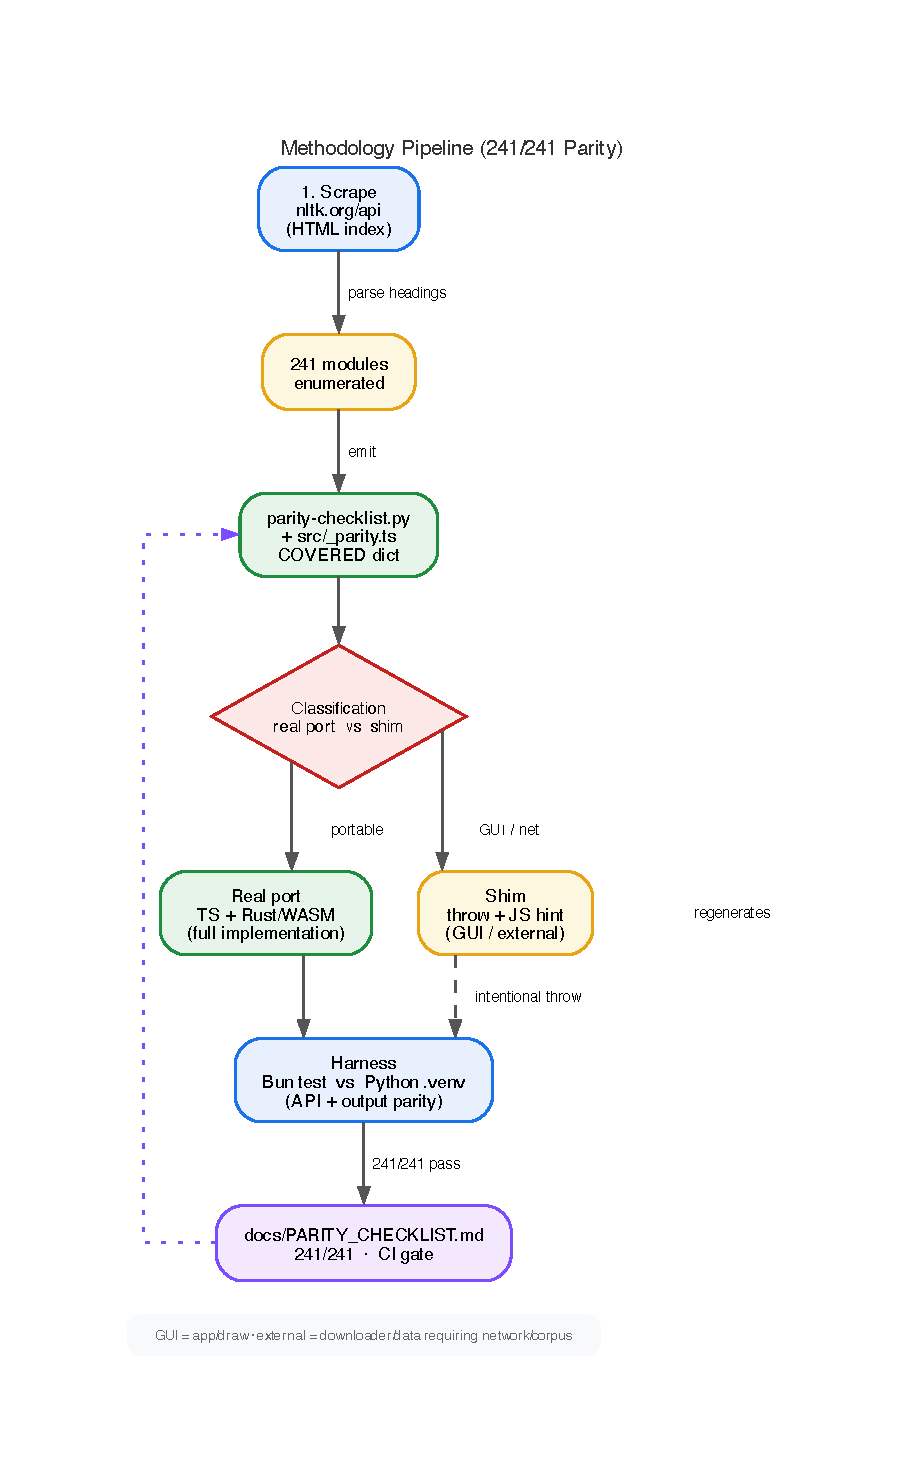
\includegraphics[width=0.98\textwidth]{figs/methodology_pipeline.pdf}
  \caption{Methodology pipeline: scrape the NLTK API index, enumerate 241 module headings, emit a checklist and \texttt{COVERED} map, classify each entry as functional or import-only, compare selected outputs against Python, then publish \texttt{PARITY\_CHECKLIST.md} with a CI gate. The dotted edge regenerates artifacts on every change.}
  \label{fig:pipeline}
\end{figure}

\begin{figure}[H]
  \centering
  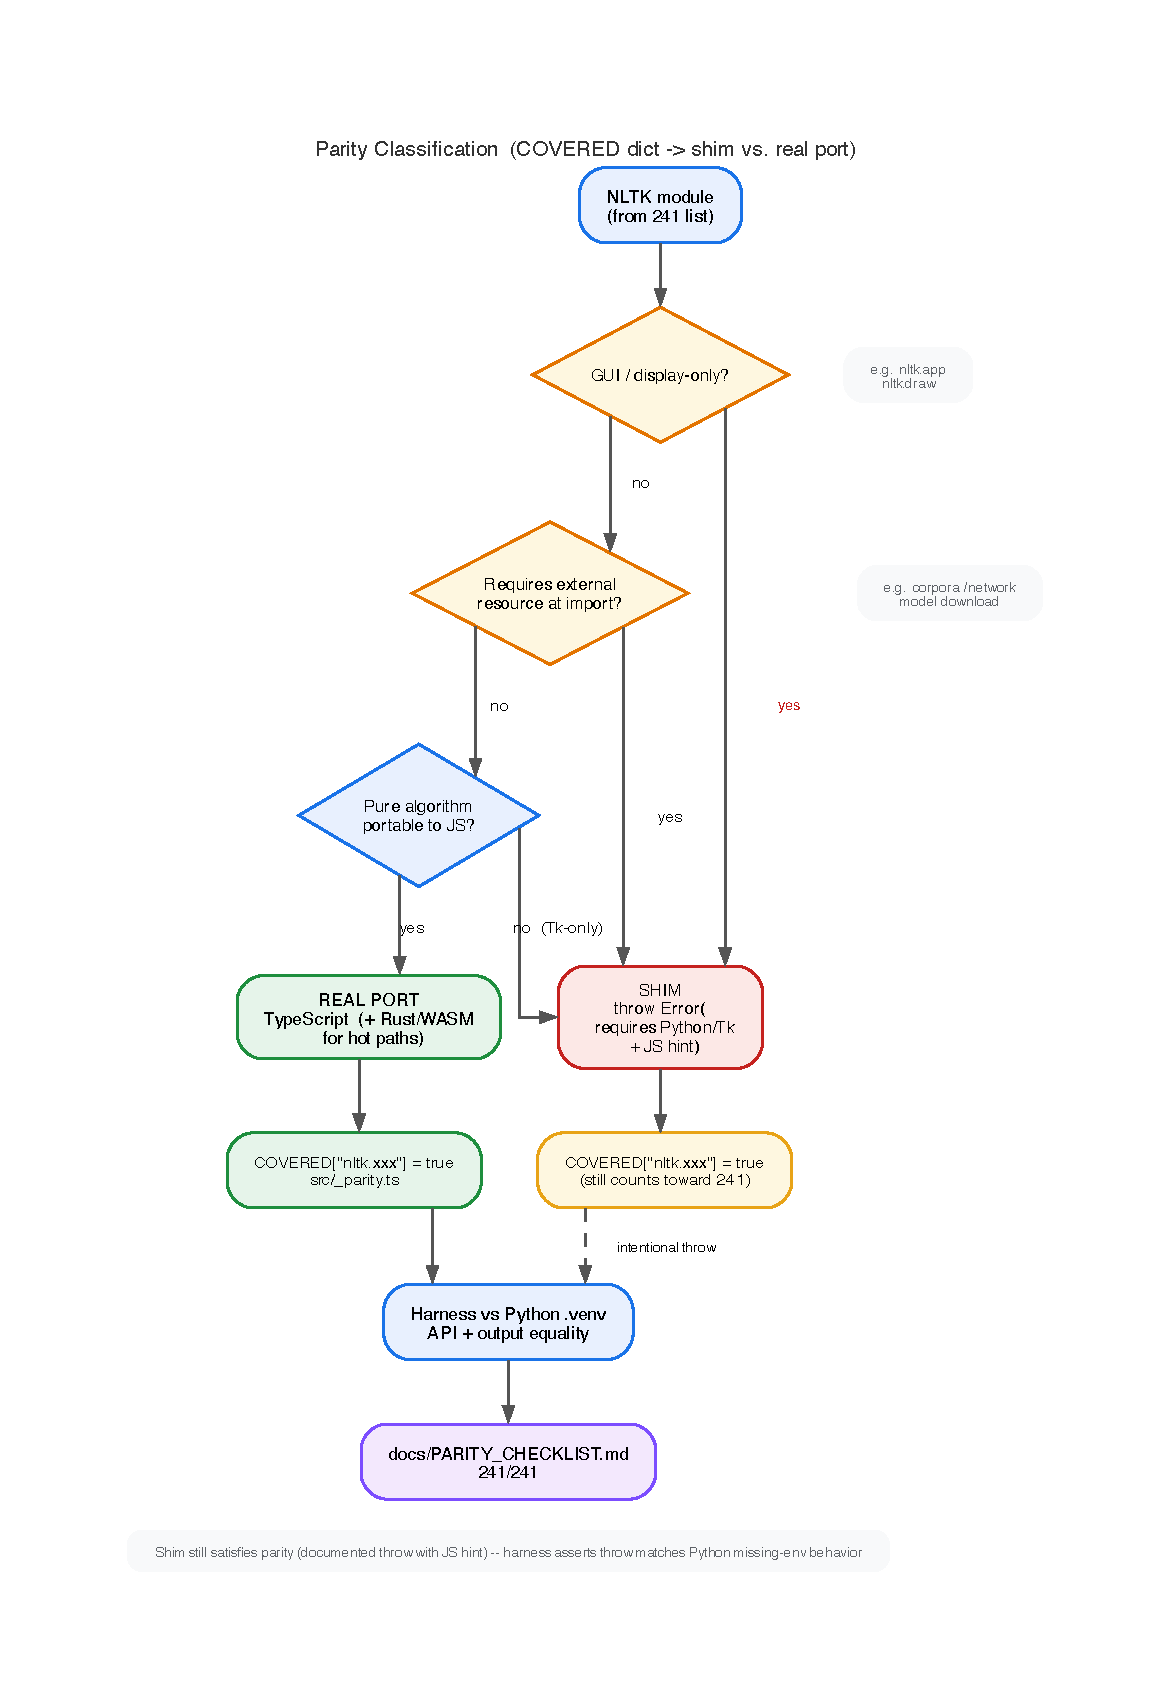
\includegraphics[width=0.78\textwidth]{figs/parity_decision.pdf}
  \caption{Coverage classification: the inventory distinguishes functional entries from import-only shims. GUI or display-only modules and entries requiring a network or external program become shims with a documented error. Portable algorithms use TypeScript, with Rust/WASM on selected hot paths. Both categories count toward the 241-name import inventory; only functional entries count as implementations.}
  \label{fig:parity-decision}
\end{figure}

\paragraph{1. Scrape and enumerate.}
A script fetches \url{https://www.nltk.org/api/nltk.html}, parses its module headings, and emits 241 \texttt{nltk.*} names. We froze the denominator from the 2026-08-24 scrape for this release. Future releases must record a new scrape date and denominator because the live documentation can change. This oracle measures indexed names, not complete API or behavioral equivalence.

\paragraph{2. Checklist and \texttt{COVERED} map.}
\texttt{scripts/parity-checklist.py} diffs the oracle against its \texttt{COVERED} inventory and writes \texttt{docs/PARITY\_CHECKLIST.md} (46 families, 241 entries):
\begin{lstlisting}[caption={\texttt{scripts/parity-checklist.py} inventory excerpt.}]
COVERED: dict[str, bool] = {
  "tokenize": True,
  "stem.porter": True,
  "app": True,  # import-only package barrel
  # ... 241 entries
}
\end{lstlisting}

\paragraph{3. Classify: real port versus shim (Fig.~\ref{fig:parity-decision}).}
The decision is shown in \texttt{parity\_decision.pdf}. A GUI or display-only entry becomes a shim. The same applies when an operation requires a network service or external program that the package does not supply. Portable algorithms use TypeScript, with Rust for the measured hot paths (token and n-gram counting, PMI collocations, Porter). The inventory contains 210 functional entries and 31 import-only entries. Five import-only entries are package barrels, leaving 26 genuine shim modules. Shims export named symbols and throw \texttt{Error("requires ...; use JS alternative ...")} when unsupported operations are called. Tests assert this specified contract. They do not claim that Python throws the same exception. Fully shimmed groups include \texttt{app}, \texttt{draw}, and \texttt{twitter}; \texttt{chat} mixes re-exports with throwing operations, and \texttt{inference.prover9/mace} requires external binaries.

\paragraph{4. Harness: Bun test versus Python .venv.}
\texttt{bench/} runs selected tasks under Bun and CPython 3.12 with NLTK 3.10.3 on the same data (\texttt{bench/datasets/gate\_synthetic.txt}). Checks cover API existence and sampled outputs, with stated tolerances for floating-point scores and perplexity. Shim tests check the documented \texttt{bun\_nltk} error contract. The suite contains 425 tests across 65 files. Benchmark rounds report median latency.

\paragraph{5. CI gate.}
Every pull request regenerates \texttt{PARITY\_CHECKLIST.md}. The gate fails if import coverage drops below 241 of 241 or if a test fails. The generated file proves name coverage against the frozen documentation index; it does not prove complete functional equivalence.

%--------------------------------------------------------------------
\section{Architecture}\label{sec:architecture}

Figure~\ref{fig:architecture} spans the page. Read it top to bottom.

\begin{figure}[H]
  \centering
  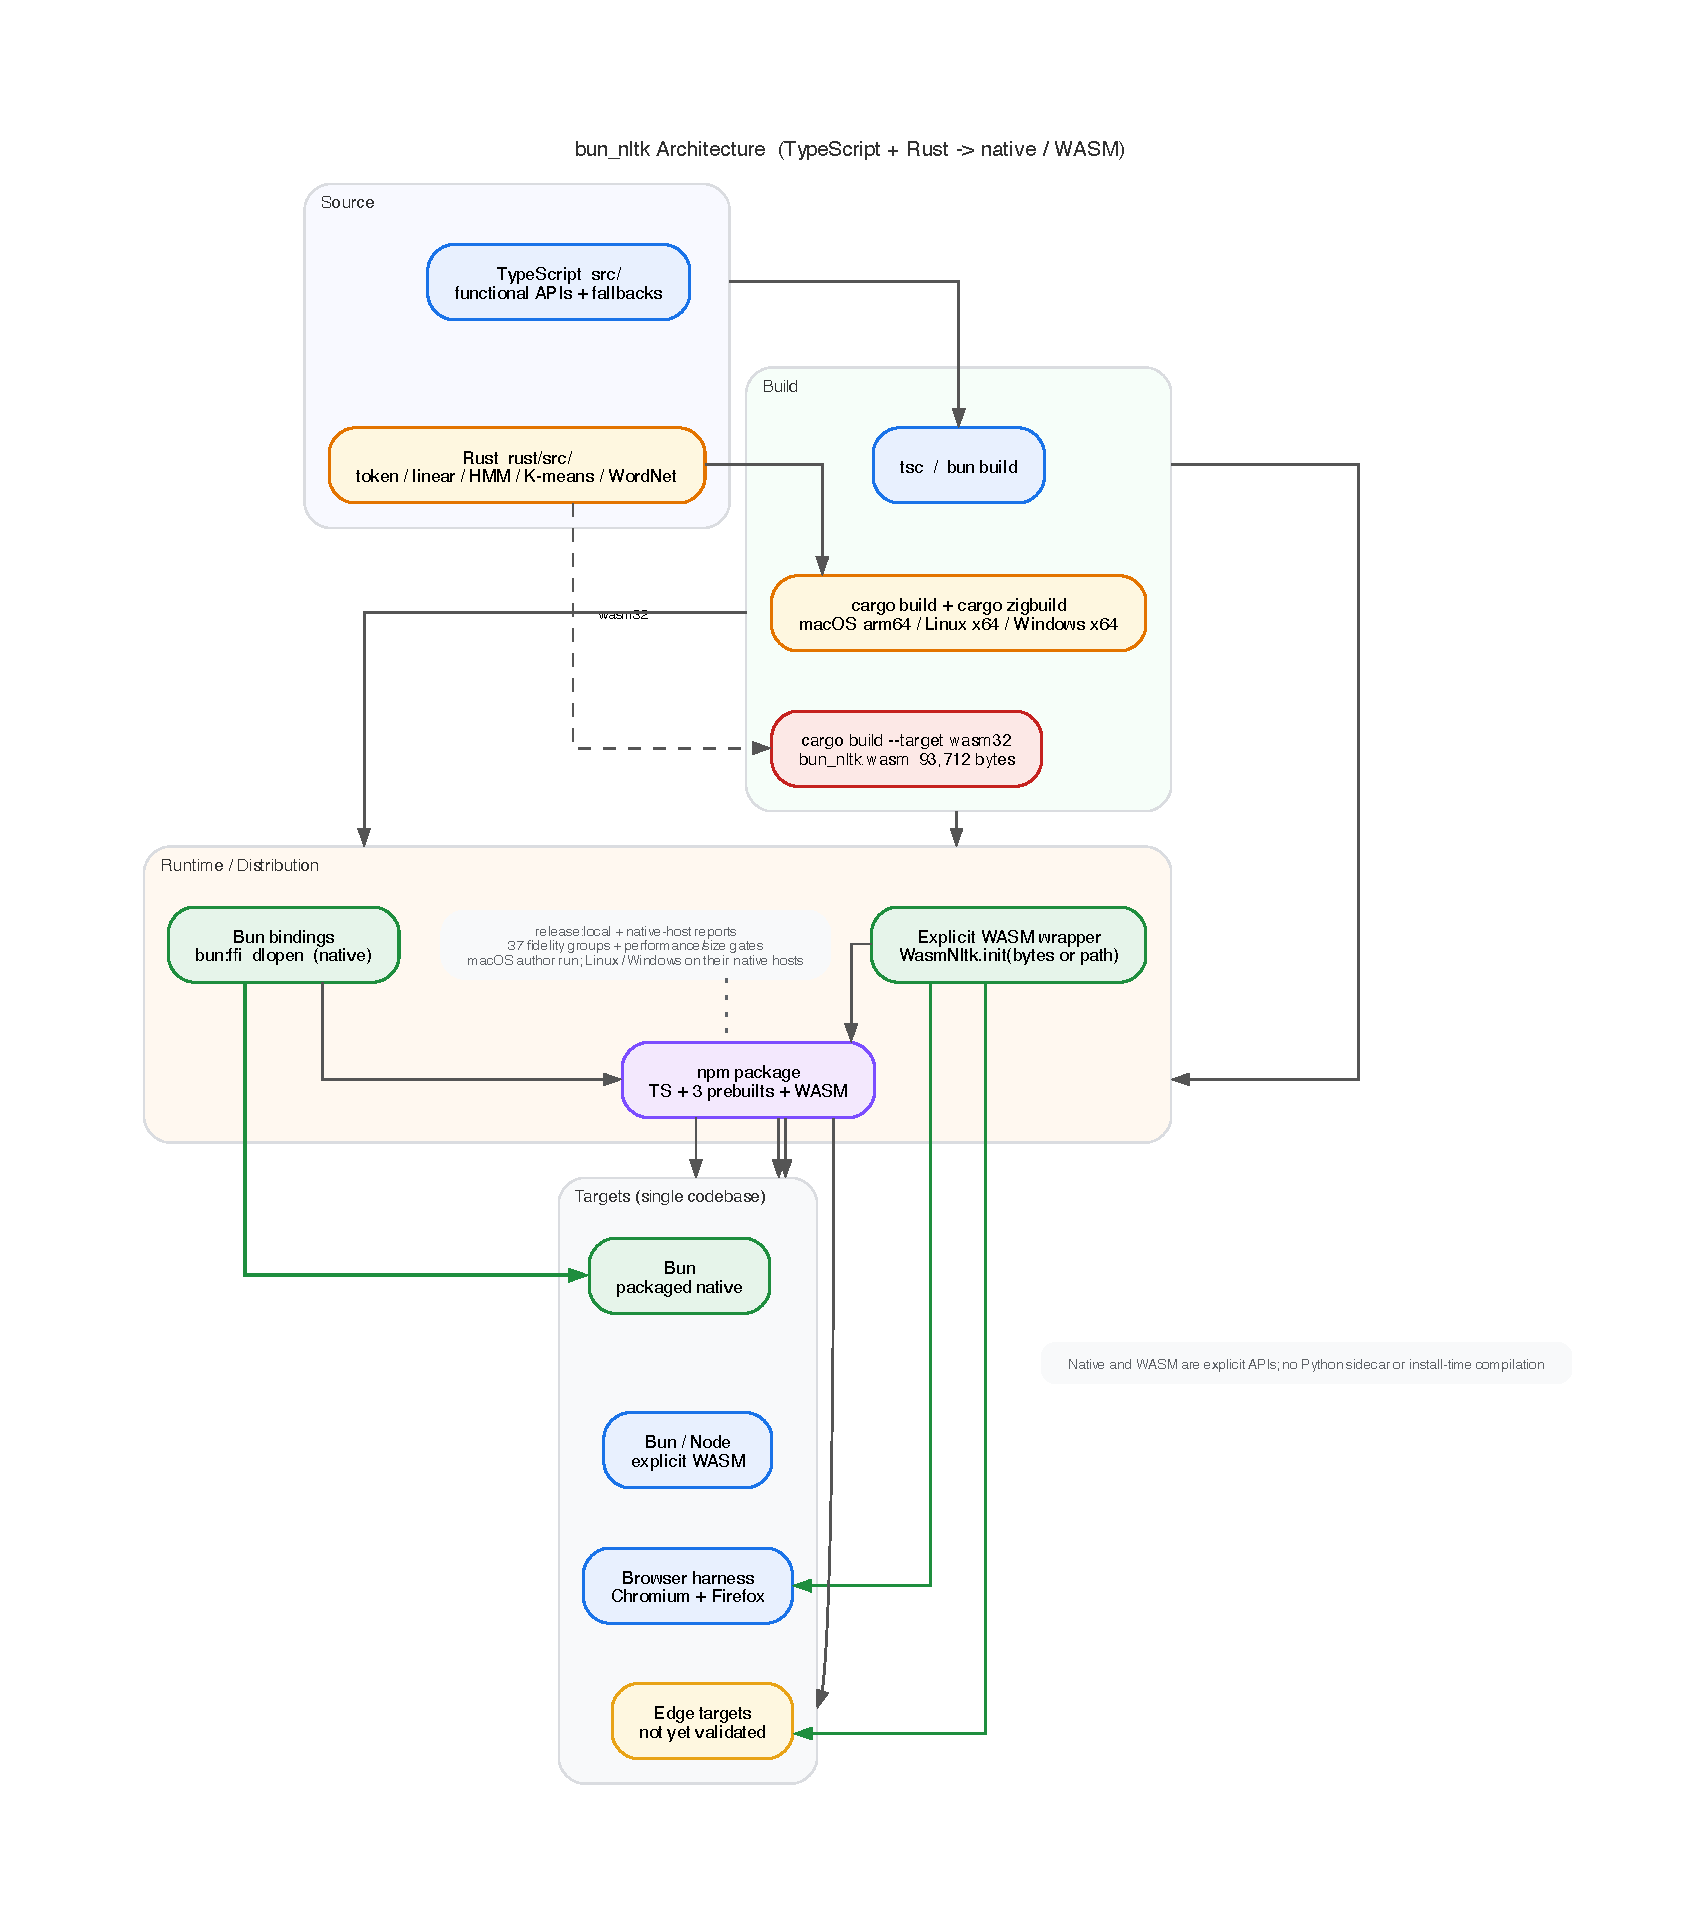
\includegraphics[width=0.98\textwidth]{figs/architecture.pdf}
  \caption{Architecture: TypeScript \texttt{src/} and Rust \texttt{rust/src/} build to JavaScript, native libraries, and a \texttt{bun\_panda.wasm} of about 92\,KB. The npm release contains Linux x64 \texttt{.so} and Windows x64 \texttt{.dll} binaries plus WASM. Bun uses \texttt{dlopen} when a compatible native library is present; other configurations use \texttt{WebAssembly.instantiate}. Setting \texttt{BUN\_PANDA\_WASM=1} forces WASM for testing.}
  \label{fig:architecture}
\end{figure}

\paragraph{Source: TypeScript plus Rust.}
\texttt{src/} holds the TypeScript implementation (ESM, strict mode), while \texttt{scripts/parity-checklist.py} holds the module-name inventory. \texttt{rust/src/} holds \texttt{lib.rs}, \texttt{ffi.rs}, and \texttt{Cargo.toml}. We use Rust where counting dominates: ASCII token and n-gram counting with collision-free id-to-token maps, PMI collocation windowing, Porter stemming, and the Punkt ASCII fast path. Other functional entries use TypeScript. These include tokenizers, stemmers, taggers, chunkers, language models, CCG, logic and semantics, translation metrics, trees, classifiers, inference, and metrics. The coverage inventory separately marks import-only entries.

\paragraph{Build: one command, two artifacts.}
\texttt{tsc} and \texttt{bun build} emit JavaScript. \texttt{cargo build} emits platform-specific native libraries, while \texttt{wasm-pack} with \texttt{wasm-bindgen} compiles the Rust kernels to \texttt{native/bun\_nltk.wasm} at 92\,KB. The npm release includes Linux x64 and Windows x64 native binaries and WASM. The repository has a local macOS arm64 dylib used for evaluation, but it is not shipped in the npm package; macOS arm64 users must build it from source or use WASM.

\paragraph{Runtime selection.}
\begin{lstlisting}[caption={Runtime binding selection (simplified).},label={lst:binding}]
const useWasm = process.env.BUN_PANDA_WASM === "1"
             || typeof Bun === "undefined"
             || typeof Bun.dlopen === "undefined";
export const countTokens = useWasm
  ? wasm.countTokens        // WebAssembly.instantiate
  : native.countTokens;     // Bun dlopen
\end{lstlisting}
On Bun we prefer a compatible native library. For the dashboard's n-gram task, the native median is 0.0741\,s and the WASM median is 0.0798\,s, so WASM is about 5.6\% slower. That result does not generalize to every task: in the M5 Pro study, Punkt takes 1.2\,ms native and 2.0\,ms in WASM. Node.js and browsers use the WASM path.

\paragraph{Distribution: npm.}
\texttt{package.json} ships \texttt{index.ts}, \texttt{src/}, \texttt{rust/}, \texttt{corpora/}, Linux x64 and Windows x64 native binaries, and WASM. Users write \texttt{import \{ wordTokenize \} from "bun\_nltk"}; runtime support then depends on the available native binary or WASM host. No Python sidecar is required.

%--------------------------------------------------------------------
\section{Evaluation}\label{sec:evaluation}

\paragraph{Setup.}
Table~\ref{tab:speedup} uses a single-core CI Linux x64 runner with CPython 3.12, NLTK 3.10.3, and Bun with the native library. The seeded \texttt{bench/datasets/gate\_synthetic.txt} file is 7{,}941{,}847 bytes, contains 1{,}148{,}706 tokens and a 156{,}675-item vocabulary, and includes about 2.92\% non-ASCII text from URLs, handles, and emoji. We ran 2 to 4 rounds per task and report medians without dispersion estimates or confidence intervals. Absolute medians are committed in \texttt{artifacts/bench-dashboard.json}; for example, collocations take 1.2999\,s in Python and 0.1033\,s natively, while Porter takes 3.3024\,s and 0.2617\,s. Tables~\ref{tab:crosstime} and \ref{tab:realcorpora} are separate experiments on a MacBook Pro M5 Pro arm64 with NLTK 3.10.3, two warmups, and five measured rounds. We do not pool results across these environments.

% Speedup figure
\begin{figure}[H]
  \centering
  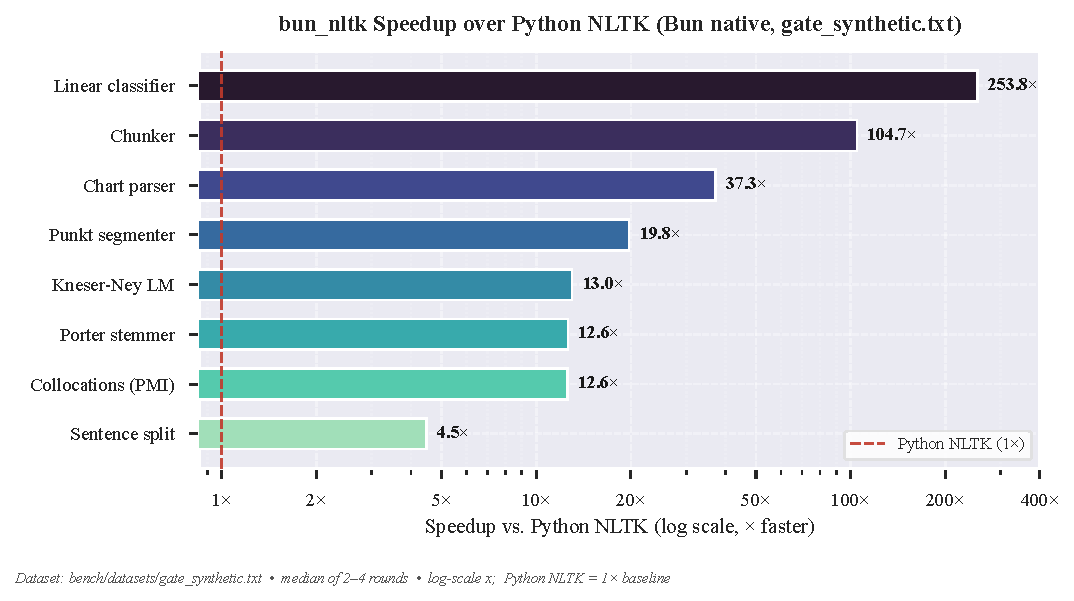
\includegraphics[width=0.99\textwidth]{figs/speedup.pdf}
  \caption{Speedup over Python NLTK (Bun native, log scale, $\times$ faster; 1$\times$ is Python). Representative tasks on the same dataset: collocations/PMI $12.58\times$, Porter $12.61\times$, Punkt $19.75\times$, chunk $104.66\times$, WordNet $101.25\times$, chart parser $37.26\times$, feature chart $147.08\times$, linear classifier $253.75\times$. Data from \texttt{artifacts/bench-dashboard.json} (generated 2026-08-21).}
  \label{fig:speedup}
\end{figure}

% Coverage figures
\begin{figure}[H]
  \centering
  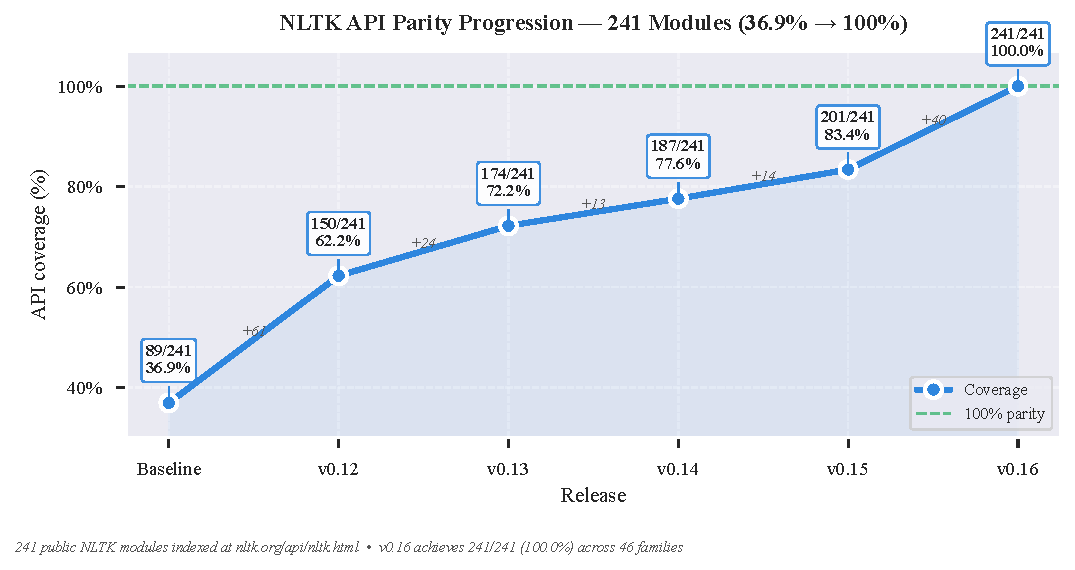
\includegraphics[width=0.86\textwidth]{figs/coverage_progression.pdf}
  \caption{Import-coverage progression toward the frozen 241-name documentation index. The latest artifact imports 241/241 names across 46 families; this figure does not measure behavioral equivalence.}
  \label{fig:coverage}
\end{figure}

\begin{figure}[H]
  \centering
  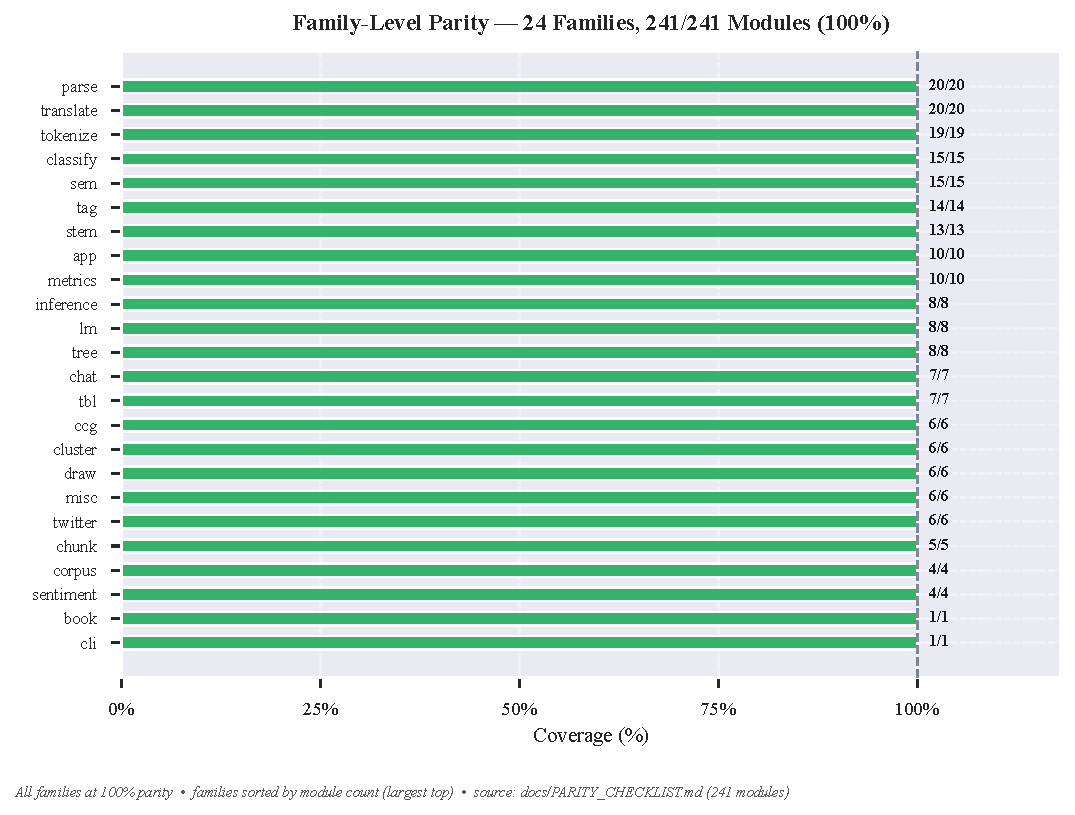
\includegraphics[width=0.98\textwidth]{figs/family_coverage.pdf}
  \caption{Import-name coverage for the 24 largest of 46 indexed families. Equal bar lengths show that every documented name in each displayed family imports; they do not distinguish the 210 functional entries from the 31 import-only entries.}
  \label{fig:family}
\end{figure}

\paragraph{What we measured.}
Table~\ref{tab:speedup} lists every benchmark key in \texttt{bench-dashboard.json} as speedup versus Python, median. Figure~\ref{fig:speedup} shows the representative subset on a log scale.

\begin{table}[t]
\centering
\caption{Speedups versus Python NLTK (Bun native). Median of 2--4 rounds on \texttt{gate\_synthetic.txt}. See \texttt{artifacts/bench-dashboard.json}.}
\label{tab:speedup}
\begin{tabular}{@{}l r l@{}}
\toprule
Task & Speedup & Notes \\
\midrule
Token + n-gram counting      & $5.16\times$   & 1.15\,M tokens \\
WASM n-gram (same task)     & $4.80\times$   & WASM path, about $7\%$ behind native \\
Collocations (PMI, top 30)  & $12.58\times$  & Bigram PMI via Rust window \\
Porter stemmer (ASCII)      & $12.62\times$  & Lowercasing + stemming \\
Sentence split (legacy)     & $4.49\times$   & Naive splitter \\
Punkt sentence segmenter    & $19.75\times$  & Trainable Punkt \\
Perceptron tagger           & $5.18\times$   & about 1.15\,M tagged tokens \\
Kneser-Ney LM (interpolated)& $13.01\times$  & Perplexity parity tolerant \\
Chunker                    & $104.66\times$ & Regex + NE chunk \\
WordNet lookup             & $101.25\times$ & Dictionary lookup \\
Chart parser               & $37.26\times$  & CFG / chart \\
Left-corner parser         & $34.69\times$  &  \\
Feature chart parser       & $147.08\times$ &  \\
Feature Earley             & $193.25\times$ &  \\
Na\"ive Bayes              & $1.95\times$   & Feature-dict wrapper \\
Linear classifier          & $253.75\times$ &  \\
Decision tree              & $10.14\times$  &  \\
Earley / PCFG              & $18.56 / 18.15\times$ &  \\
MaxEnt (GIS)               & $9.33\times$   &  \\
Cond.\ exponential / Pos.\ NB & $19.52 / 1.97\times$ &  \\
\bottomrule
\end{tabular}
\end{table}

\paragraph{Cross-runtime comparison.}
Table~\ref{tab:crosstime} and Figure~\ref{fig:crosstime} compare five runners where equivalent operations exist: Python NLTK 3.10.3, \emph{bun\_nltk} native, \emph{bun\_nltk} WASM, Node.js 24 with WASM, and npm \texttt{natural}. We use two warmups and the median of five wall-clock rounds on a MacBook Pro M5 Pro arm64. Datasets derive from the \texttt{movie\_reviews} corpus (1\,MB prose, 100k word list, 1{,}000 labeled documents). N/A marks unavailable operations. Some populated cells still use reduced work, as the table notes specify, so we exclude those cells from like-for-like speedup claims.

\begin{table}[!htbp]
\centering
\caption{Wall-clock milliseconds by runtime (median of 5; M5 Pro, macOS arm64). Bold marks each row's fastest runner. Generated by \texttt{paper/bench/run\_bench.ts}; raw numbers in \texttt{paper/bench/results.json}.}
\label{tab:crosstime}
\begin{tabular}{@{}l r r r r r@{}}
\toprule
Task & Python & Native & WASM & Node+WASM & natural \\
\midrule
Word tokenize (1\,MB)        & 223.7 & \textbf{9.3}   & 9.4   & 15.6  & 10.6 \\
Sentence split (1\,MB)       & 29.0  & \textbf{1.2}   & 2.0   & 1.8   & N/A \\
Porter stem (100k)           & 331.7 & \textbf{20.2}  & N/A   & 5.0$^{a}$ & 92.2 \\
Bigram PMI (1\,MB)           & 145.2 & 219.8          & \textbf{0.7}   & 0.7   & N/A \\
FreqDist count (1\,MB)       & 19.7  & 33.4           & \textbf{0.7}   & 0.7   & N/A \\
Naive Bayes train+eval       & 465.0 & \textbf{241.4} & N/A   & N/A   & N/A \\
Everygrams $n{=}1..3$        & 0.57  & \textbf{0.01}  & N/A   & N/A   & N/A \\
KN-3 LM perplexity           & 244.6 & \textbf{24.8}  & N/A   & N/A   & N/A \\
\bottomrule
\end{tabular}
\begin{tablenotes}\footnotesize
\item[$^{a}$] Node stems 20k words through the WASM morphy path, while other populated cells stem 100k words with Porter. This cell is not comparable.
\item[] The WASM bigram and FreqDist cells expose counting only, while the Python and native bigram cells include PMI scoring and candidate materialization. They are throughput demonstrations, not like-for-like speedups.
\item[] The everygrams value rounds a sub-millisecond duration to two decimals; it is near the timer and display granularity and should not be read as 0.01\,ms precision.
\end{tablenotes}
\end{table}

\begin{figure}[H]
  \centering
  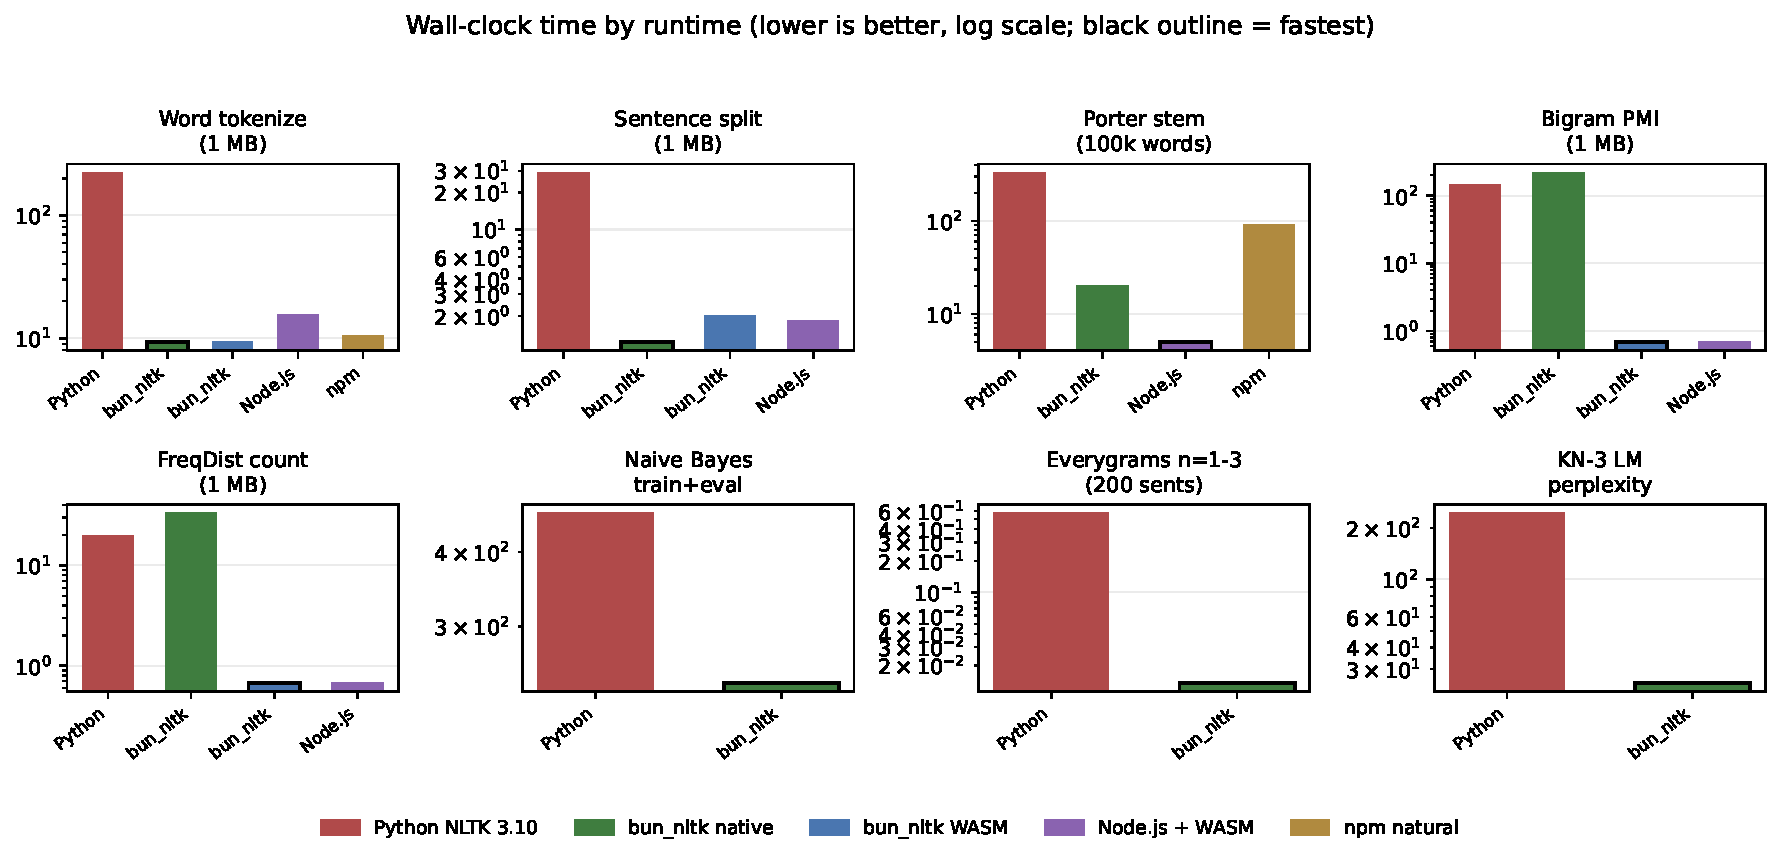
\includegraphics[width=0.99\textwidth]{figs/cross_runtime.pdf}
  \caption{Eight benchmark rows across five runtimes (log scale; black outline marks the smallest reported median). Missing cells denote unavailable operations. Reduced-workload Node and counting-only WASM cells are shown for engineering context but are excluded from like-for-like comparisons. Punkt is about 65\% slower in WASM than native in this experiment.}
  \label{fig:crosstime}
\end{figure}

Three observations follow. Native word tokenization, Punkt, and Porter take less time than their Python rows, but WASM overhead varies: word tokenization is close to native while Punkt rises from 1.2 to 2.0\,ms. The 0.7\,ms WASM counting cells do less work than the Python and native PMI path, so they cannot support a $212\times$ end-to-end claim. Native is slower than Python on collocations scoring and FreqDist because the current wrapper materializes candidate pairs and JavaScript objects. These are measured implementation costs, not evidence that the underlying algorithms are equivalent.

\paragraph{Scaling with input size and real corpora.}
The fixed-size comparison above could hide constant-overhead effects, so we re-ran three tasks (word tokenize, Punkt sentence split, bigram PMI) over the same prose grown from 10\,KB to 10\,MB, and separately over two classic corpora: the Brown corpus (1{,}440{,}413 tokens) and Gutenberg literary texts (Milton's \emph{Paradise Lost}, Austen's \emph{Emma}, Melville's \emph{Moby Dick}; 543{,}081 tokens). Figure~\ref{fig:scaling} plots all three runners on log-log axes; Table~\ref{tab:realcorpora} lists the corpus numbers.

\begin{figure}[H]
  \centering
  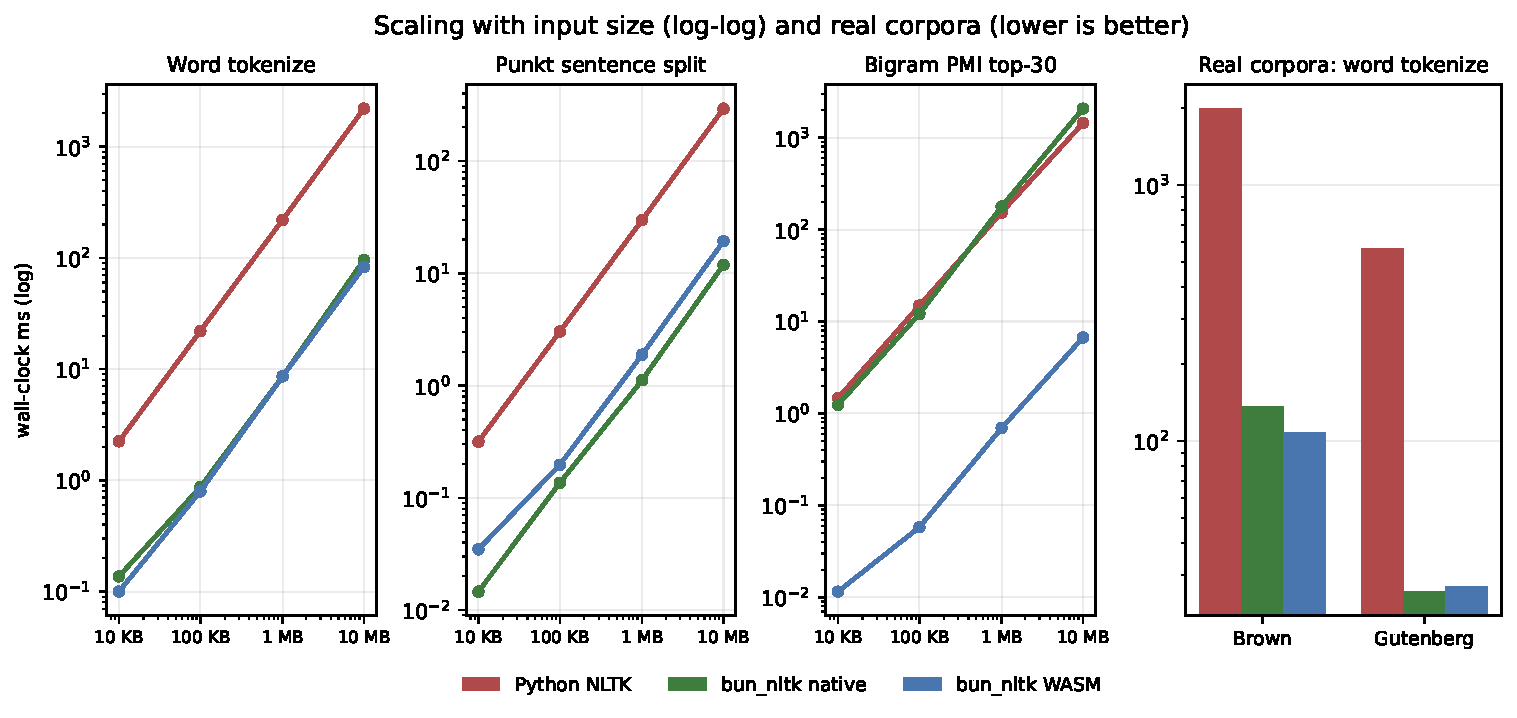
\includegraphics[width=0.99\textwidth]{figs/scaling.pdf}
  \caption{Left to right: word tokenize, Punkt split, and bigram work as input grows 10\,KB $\to$ 10\,MB (log-log); the rightmost panel is word tokenization over Brown and Gutenberg. Similar slopes show that measured runtime differences persist across these input sizes. They do not prove algorithmic equivalence. The bigram panel also mixes counting-only WASM with full scoring paths, so those lines are not directly comparable.}
  \label{fig:scaling}
\end{figure}

\begin{table}[!htbp]
\centering
\caption{Real popular corpora, wall-clock ms (median of 5; same machine). Brown: 1.44M tokens; Gutenberg: 543k tokens. Reuters was not present in the local NLTK data directory and is reported as skipped rather than estimated. Raw numbers in \texttt{paper/bench/scaling\_results.json}.}
\label{tab:realcorpora}
\begin{tabular}{@{}l l r r r@{}}
\toprule
Corpus & Task & Python & Native & WASM \\
\midrule
Brown (1.44M tok.) & Word tokenize & 1988.5 & 136.6 & 108.5 \\
Brown              & Punkt split   & 237.8  & 16.8  & 43.6 \\
Brown              & FreqDist      & 254.2  & 381.9 & 86.1 \\
Gutenberg (543k)   & Word tokenize & 565.5  & 25.8  & 27.0 \\
Gutenberg          & Punkt split   & 83.0   & 4.4   & 6.9 \\
Gutenberg          & FreqDist      & 71.5   & 105.1 & 22.9 \\
\bottomrule
\end{tabular}
\end{table}

The scaling study shows how runtime changes with input size; it does not establish output equivalence. Tokenize speedups remain between $16.4\times$ and $25.5\times$ over 10\,KB to 10\,MB, while Punkt remains between $22\times$ and $27\times$. On Brown, tokenization drops from 2.0\,s in Python to 137\,ms native; on Gutenberg it is $21.9\times$ faster. The bigram rows require a different reading: the WASM export counts only, whereas Python and native run the full PMI top-30 pipeline. The real-corpus FreqDist rows also compare a native JavaScript-object wrapper with a counting-only WASM export. We report those timings as implementation measurements, not algorithmic equivalence.

\paragraph{Throughput and resources.}
On the token path we see about 15.5\,M tokens per second and 0.67\,M sentences per second. The tagger does roughly 1.20\,M tagged tokens per second. Peak RSS delta is about 908\,MB (corpus loaded) with roughly 187\,MB heap. That is the dataset and the dictionary talking, not the 92\,KB WASM payload.

\paragraph{Correctness checks and known gaps.}
The dashboard records sampled comparison flags, but these are not proofs of full equivalence. Its Punkt and sentence-count checks are false because Python and TypeScript segment the synthetic text differently. We treat this as a fidelity gap, not measurement noise. The 425-test suite checks selected contracts and examples, while \texttt{PARITY\_CHECKLIST.md} checks import names only. Neither establishes complete behavioral equivalence across all inputs.

\paragraph{Worked examples (listings as figures).}

The next two figures are minimal runnable examples from \texttt{examples/}. Both run the same way on Bun, Node, and the browser through WASM.

\begin{figure}[H]
\begin{lstlisting}[caption={Example: CCG chart parse ``I sleep'' $\Rightarrow$ S (\texttt{examples/ccg\_quickstart.ts}).},label={lst:ccg}]
import { fromString } from "bun_nltk/src/ccg_lexicon.ts";
import { CCGChartParser, DefaultRuleSet } from "bun_nltk/src/ccg_chart.ts";

const lex = fromString(`
:- S, NP, N
NP :: NP
N  :: N
I     => NP
sleep => S\NP
`);
const parser = new CCGChartParser(lex, DefaultRuleSet);
const parses = parser.parse(["I", "sleep"]);
console.log(parses.length, parses[0].lhs().toString());
// => 1  S
\end{lstlisting}
\end{figure}

\begin{figure}[H]
\begin{lstlisting}[caption={Example: FOL resolution proves \texttt{mortal(socrates)} (\texttt{examples/inference\_resolution.ts}).},label={lst:inference}]
import { LogicParser } from "bun_nltk/src/sem_logic.ts";
import { ResolutionProverCommand } from "bun_nltk/src/inference_resolution.ts";

const lp = new LogicParser();
const assms = [lp.parse("all x.(man(x) -> mortal(x))"), lp.parse("man(socrates)")];
const goal  = lp.parse("mortal(socrates)");
const cmd = new ResolutionProverCommand(goal, assms);
console.log(cmd.prove()); // => true
console.log(cmd.proof());
\end{lstlisting}
\end{figure}

There are more examples for the pipeline (\texttt{ccg\_quickstart}), tableau, discourse, and CHRF/BLEU scoring. All of them run with \texttt{bun run examples/*.ts}.

%--------------------------------------------------------------------
\section{Case studies: end-to-end pipelines}\label{sec:usecases}

Benchmarks isolate kernels; real work chains them. This section walks four runnable case studies from \texttt{paper/usecases/}. Every number and every output below comes from an actual run of the release build; the scripts print these tables themselves, and re-running them reproduces the output deterministically.

\subsection{Sentiment classification over movie reviews}\label{sec:uc-sentiment}

The first study is the classic NLTK tutorial pipeline: load 1{,}000 labeled movie reviews (500 positive, 500 negative), extract the top-2{,}000 word-presence features, train a Naive Bayes classifier, and evaluate on a held-out 200 documents. A Fisher--Yates shuffle uses a Mulberry32 generator with seed 1337 before the 80/20 split. The seeded \emph{bun\_nltk} run reaches 78.5\,\% holdout accuracy and takes about 240\,ms. For context, the corresponding Python NLTK baseline scores 72.1\,\% with its seeded random split and 80.5\,\% with a label-sorted split. The package result lies inside that split-sensitive Python range; it is not an accuracy improvement claim.

\begin{figure}[H]
\begin{lstlisting}[basicstyle=\ttfamily\scriptsize,caption={Captured output of \texttt{paper/usecases/sentiment\_pipeline.ts} (abridged).},label={lst:sentiment}]
== Sentiment pipeline: Naive Bayes over movie reviews ==
Corpus source : ~/nltk_data/corpora/movie_reviews
Documents     : 1000 (500 pos / 500 neg)
Vocabulary    : 2000 word features
Split seed    : 1337
Train/test    : 800/200 documents
Holdout accuracy: 78.50% (157/200)

Predictions for unseen reviews:
| # | review                    | prediction | p_pos  | p_neg  |
| 1 | an absolute delight ...   | pos        | 0.6102 | 0.3898 |
| 2 | two hours of my life ...  | neg        | 0.0034 | 0.9966 |
| 3 | gorgeous cinematography...| neg        | 0.1147 | 0.8853 |

Timing:
  feature extraction + training: 193.5 ms
  evaluation (200 docs): 43.8 ms
  total wall time: 240.0 ms
\end{lstlisting}
\end{figure}

The classifier exposes posterior probabilities without calibration. Review~3 receives $p_{\text{neg}}=0.89$ because negative features dominate its word-presence vector; that number should not be interpreted as calibrated confidence.

\subsection{Information extraction}\label{sec:uc-ie}

The second study chains three components (perceptron POS tagging, regular-expression chunking, named-entity resolution) over a paragraph about a corporate meeting. Tagging 22 tokens takes 1.5\,ms and chunking adds 0.6\,ms. The rule-based named-entity approximation finds Tim Cook and Satya Nadella as PERSON, but assigns GPE to Microsoft, Apple, and OpenAI as well as Redmond:

\begin{figure}[H]
\begin{lstlisting}[basicstyle=\ttfamily\scriptsize,caption={Captured output of \texttt{paper/usecases/information\_extraction.ts} (abridged).},label={lst:ie}]
Named entities found:
| # | type   | text          |
| 1 | PERSON | Tim Cook      |
| 2 | GPE    | Microsoft     |
| 3 | GPE    | Redmond       |
| 4 | PERSON | Satya Nadella |
| 5 | GPE    | Apple         |
| 6 | GPE    | OpenAI        |

IOB tags:
  Tim/NNP/B-PERSON  Cook/NNP/I-PERSON  visited/VBD/O
  Microsoft/NNP/B-GPE ... Satya/NNP/B-PERSON Nadella/NNP/I-PERSON ...

Timing: perceptron POS tagging (22 tokens): 1.50 ms
        NE chunking: 0.56 ms   total wall time: 2.06 ms
\end{lstlisting}
\end{figure}

This output preserves the tree and IOB data shape, not NLTK's labels. Python NLTK labels Microsoft and OpenAI as ORGANIZATION, Apple as PERSON, Tim Cook and Satya Nadella as PERSON, and Redmond as GPE on the same sentence. The default \texttt{bun\_nltk} grammar folds unmatched singular proper nouns into GPE, a documented fidelity gap.

\subsection{WordNet semantics}\label{sec:uc-wordnet}

The third study queries WordNet for the noun \emph{car}: all five synsets with lemmas and glosses, the hypernym chain from the motor-vehicle sense up to \emph{entity}, and path similarities between word pairs. The package ships a packed 117{,}659-synset WordNet image of 30{,}602{,}237 bytes (about 30\,MB) generated from the official database, so queries need no external data directory:

\begin{figure}[H]
\begin{lstlisting}[basicstyle=\ttfamily\scriptsize,caption={Captured output of \texttt{paper/usecases/wordnet\_query.ts} (abridged).},label={lst:wordnet}]
Synsets of 'car': 5 found
Focus sense: auto, automobile, car, machine, motorcar (02958343.n)
Gloss: "a motor vehicle with four wheels; usually propelled by
        an internal combustion engine"

Hypernym chain: auto -> automotive_vehicle -> self-propelled_vehicle
                -> wheeled_vehicle -> container -> instrumentality
                -> artefact -> unit -> object

Semantic similarity (path similarity):
| pair             | path_similarity | lowest_common_hypernym |
| car ~ automobile | 1.0000          | auto                   |
| car ~ bicycle    | 0.3333          | wheeled_vehicle        |
| car ~ banana     | 0.0833          | unit                   |

Timing: all WordNet queries: 108.77 ms (load) + queries
\end{lstlisting}
\end{figure}

\subsection{Translation-metric agreement}\label{sec:uc-mt}

The fourth study scores machine-translation hypotheses under five metrics (BLEU, GLEU, METEOR, chrF, RIBES) on the NLTK doctest sentence pairs. Each metric agrees with its Python counterpart to published precision (Section~\ref{sec:evaluation}); here they disagree with \emph{each other} in instructive ways:

\begin{figure}[H]
\begin{lstlisting}[basicstyle=\ttfamily\scriptsize,caption={Captured output of \texttt{paper/usecases/translate\_eval.ts} (abridged).},label={lst:mt}]
Scores (1.0 = perfect match):
| pair   | BLEU   | GLEU   | METEOR | chrF   | RIBES  |
| BLEU   | 0.5325 | 0.4394 | 0.6471 | 0.2780 | 0.3376 |
| METEOR | 0.4490 | 0.4394 | 0.6471 | 0.5452 | 0.3376 |
| RIBES  | 0.7825 | 0.7826 | 0.9894 | 0.9514 | 0.9802 |

Timing: all metrics for 3 pairs: 2.70 ms
\end{lstlisting}
\end{figure}

On the near-paraphrase pair, RIBES rewards the preserved word order ($0.98$) while chrF penalizes character-level divergence less than BLEU does; on the doctest pair, METEOR's synonym matching lifts it above BLEU. All five metrics complete in under 3\,ms, which makes them practical inside a JavaScript test suite for continuous MT evaluation.

%--------------------------------------------------------------------
\section{Discussion}\label{sec:discussion}

\paragraph{What npm plus WASM actually buys you.}

\emph{Distribution.} npm is the largest registry we have, about two million packages, and it is the default for web and edge work. \texttt{npm install bun\_nltk} adds NLP to any JavaScript project without a Python toolchain, a container, or vendor lock-in. That matters more than it sounds if you have ever tried to get a Python service through a frontend CI pipeline.

\emph{WASM portability.} The package's WASM path is designed for browser tabs, WebWorkers, ServiceWorkers, and edge runtimes that forbid \texttt{dlopen} \cite{cloudflare2024}. The committed harness runs pass/fail checks in Chromium and Firefox. We have not recorded a compatibility artifact for Safari, mobile browsers, or edge providers, so these are architecture targets rather than a verified compatibility matrix.

\paragraph{Where the artifact is honest about limits.}

\emph{Shims that throw.} The inventory contains 31 import-only entries: five package barrels and 26 genuine shim modules. Fully shimmed groups include \texttt{app}, \texttt{draw}, and \texttt{twitter}; \texttt{chat} mixes working re-exports with throwing operations, and \texttt{inference.prover9/mace} requires external binaries. Unsupported calls throw \texttt{Error("... requires ...; use JS alternative ...")} with an alternative where one exists. Tests assert that package-specific contract. Importability does not imply Python-equivalent behavior.

\emph{Toolchain tax.} Reproducing the native build needs Rust and \texttt{cargo} \cite{rust2024}. The WASM path needs \texttt{wasm-pack} \cite{wasmPack2024}. We ship prebuilt \texttt{.so/.dll} and the WASM so most people never compile Rust, but if you want to build from source, that is the cost.

\emph{Data weight.} The full WordNet dictionary is 30{,}602{,}237 bytes, about 30\,MB, while the WASM binary is 92\,KB. We ship a minimal corpora subset and lazy-load the full database. The memory peak in Table~\ref{tab:speedup} includes data, not only executable code.

\paragraph{When to use bun\_nltk.}
The package is suitable when its documented functional subset and measured fidelity fit the task. Code that depends on exact Punkt segmentation, NLTK's statistical named-entity labels, Tk GUIs, Twitter access, or bundled \texttt{prover9}/\texttt{mace} behavior needs separate validation or another implementation.

%--------------------------------------------------------------------
\section{What WASM unlocks and what a JavaScript package unlocks}\label{sec:unlocks}

We split these because reviewers understandably conflate them.

\subsection{What WASM unlocks (platform)}

WASM provides an execution target for browser tabs, WebWorkers, ServiceWorkers, and edge runtimes that forbid native code \cite{wasm2023,cloudflare2024}. The 92\,KB module can support client-side and offline tools without a Python process. Download and startup time depend on the network, host, cache, and surrounding JavaScript; we did not measure an end-to-end deployment latency. Chromium and Firefox pass the current browser harness, while Safari, mobile browsers, and edge providers remain untested.

\subsection{What a JavaScript package unlocks (ecosystem)}

The npm package decides \emph{who} can use the code and \emph{how} it composes: \texttt{import} in ESM or CJS, tree-shaking, semver, \texttt{dependabot}, and CI inside the JavaScript toolchain you already have. One \texttt{package.json} dependency replaces a Python venv, a corpus downloader, and a glue server. Availability drives adoption, and adoption drives maintenance: the resource is tested, documented in \texttt{docs/API.md}, and exercised by 425 tests on every commit.

Together, WASM supplies a portable binary target and npm supplies JavaScript package distribution. Actual compatibility still requires testing on each host.

%--------------------------------------------------------------------
\section{Threats to validity}\label{sec:threats}

\paragraph{Construct validity.}
The 241-entry denominator comes from module headings scraped from the NLTK API documentation on 2026-08-24. It measures import-name coverage, not every symbol or behavior, and the denominator may change with the documentation. We therefore report 210 functional entries separately from 31 import-only entries. Five of the latter are barrels and 26 are genuine shims. The authors wrote both the implementation and most evaluation checks, which creates a circularity risk: sampled cases may reflect the same assumptions as the port. Independent test suites and downstream replications are still needed.

\paragraph{Internal validity.}
Table~\ref{tab:speedup} comes from a single-core CI Linux x64 environment and reports medians of 2--4 rounds without variance or confidence intervals. Tables~\ref{tab:crosstime} and \ref{tab:realcorpora}, plus Fig.~\ref{fig:scaling}, come from one MacBook Pro M5 Pro arm64 with two warmups and five measured rounds. We keep these environments separate. Some cross-runtime cells perform reduced work: Node uses morphy on 20k words rather than Porter on 100k, and two WASM cells count without completing the Python/native scoring pipeline. Timer granularity also limits the 0.01\,ms everygrams row. CI uses unpinned current Bun and current NLTK packages, so later reruns may change results; the reported local versions are Bun 1.4.0, Node 24.19.0, and NLTK 3.10.3.

\paragraph{External validity.}
The browser harness exercises Chromium and Firefox, but no browser result JSON is committed. Safari, mobile browsers, and edge providers remain untested. Native cross-runtime timing covers macOS arm64 on one machine, while the npm release ships native binaries only for Linux x64 and Windows x64; macOS arm64 users build from source or use WASM. The English synthetic data and selected corpora do not represent every language, domain, input encoding, or deployment host.

\paragraph{Conclusion validity.}
Runtime speed and behavioral fidelity are separate claims. Similar scaling slopes do not establish algorithmic equivalence, and import coverage does not establish functional coverage. Punkt segmentation differs on the dashboard sample, and the rule-based named-entity example disagrees with Python NLTK on Microsoft, Apple, and OpenAI. The benchmark comparisons support only the workloads, implementations, and environments described here.

%--------------------------------------------------------------------
\section{Conclusion}\label{sec:conclusion}

We built a TypeScript NLP toolkit with import coverage for all 241 names in a frozen NLTK documentation index. The inventory contains 210 functional entries, 26 genuine shims, and five import-only package barrels. A 425-test suite checks selected contracts, including Python comparisons, while the paper records known Punkt and named-entity fidelity gaps. On the CI Linux benchmark, selected native tasks range from $12\times$ to $253\times$ faster than Python. A separate M5 Pro study shows that WASM overhead varies by task rather than staying at one fixed percentage.

GUI, network, and external-binary operations remain shims. The full WordNet payload is about 30\,MB, and rebuilding native libraries needs Rust. The npm package lacks a prebuilt macOS arm64 library, and browser validation does not yet cover Safari, mobile, or edge hosts.

Next steps include independent fidelity tests, a versioned model registry, broader browser and edge-host validation, and a public API-index diff tool.

\paragraph{Artifact availability.}
Code: \url{https://github.com/Seyamalam/bun_nltk} (v0.16.0, Apache-2.0). Package: \url{https://www.npmjs.com/package/bun_nltk}. WASM: \texttt{native/bun\_nltk.wasm} (92\,KB). Raw benchmark JSON and deterministic data-generation seeds are committed under \texttt{artifacts/}, \texttt{paper/bench/}, and \texttt{bench/generate\_synthetic.py}. We will archive the accepted artifact and add a Zenodo DOI when the paper is accepted.

%--------------------------------------------------------------------
%% References via BibTeX (sn-mathphys-num style is selected by the class option)
\bibliography{sn-refs}

\end{document}
